%
% File acl2019.tex
%
%% Based on the style files for ACL 2018, NAACL 2018/19, which were
%% Based on the style files for ACL-2015, with some improvements
%%  taken from the NAACL-2016 style
%% Based on the style files for ACL-2014, which were, in turn,
%% based on ACL-2013, ACL-2012, ACL-2011, ACL-2010, ACL-IJCNLP-2009,
%% EACL-2009, IJCNLP-2008...
%% Based on the style files for EACL 2006 by 
%%e.agirre@ehu.es or Sergi.Balari@uab.es
%% and that of ACL 08 by Joakim Nivre and Noah Smith

\documentclass[11pt,a4paper]{article}
\usepackage[hyperref]{acl2019}
\usepackage{amsmath}
\usepackage{times}
\usepackage{latexsym}
\usepackage{graphicx}
\usepackage{breqn}
\usepackage{amssymb}

\usepackage{url}

\aclfinalcopy % Uncomment this line for the final submission
%\def\aclpaperid{***} %  Enter the acl Paper ID here

%\setlength\titlebox{6cm}
% You can expand the titlebox if you need extra space
% to show all the authors. Please do not make the titlebox
% smaller than 5cm (the original size); we will check this
% in the camera-ready version and ask you to change it back.

\graphicspath{{figure/}}

\newcommand\BibTeX{B\textsc{ib}\TeX}

\title{Sentiment Analysis and Deep Reinforcement Learning for Algorithmic Trading}

\author{Chi Zhang \\
  Department of Computer Science \\
  University of Southern California \\
  Los Angeles, CA, 90089 \\
  \texttt{zhan527@usc.edu} \\}

\date{}

\begin{document}
\maketitle
\begin{abstract}
  In algorithmic trading, we buy/sell stocks using computers automatically. While high frequency algorithmic trading is pretty common in financial market, we focus on long-term algorithmic trading based on historical stock price and news/tweets. To make the problem tractable, we model the transaction as a sequential decision making problem. The transaction period is one day. The return is calculated using the close price plus a fixed rate of commission.
  In this report, we divide the data processing pipeline as follows: 1) we train a sentiment analyzer by concatenating all the news of a particular day and predict the trend (up/down) of the next day. 2) we implement trading strategy based on the prediction results. We compare a na\"ive strategy versus policy trained using reinforcement learning.
  
  For sentiment analyzer, we implement multi-sized window CNN and dual attention model that incorporates temporal relationship among news data.
  We use Proximal Policy Optimization (PPO) to train policy that maximize the returns using simulated trading environment that fed with real data.
  
  We test our approaches on Dow Jones Industrial Average (DJIA) and experiments show that all the methods overfit on training dataset and the performance on testing data amounts to random guessing. We further investigate the quality of this dataset and conclude that even a human can't make good predictions given the news as observation. Our code is open source at \url{https://github.com/vermouth1992/CSCI699ml4know/tree/master/project}.
\end{abstract}


\section{Introduction}
Algorithm trading is gaining attention with the extraordinary performance of deep learning algorithms in computer vision, natural language process and sequential decision making domain \cite{high_frequency_drl}. Most algorithmic trading, however, is applied in high frequency domain (large transaction volume at fractions of a second), where the trend of stock market is stationary and easily predictable. This is generally not true in long-term investment since the underlying dynamics of stock market is constantly changing. From basic economics theory, the stock price indicates the future value of a company and reflects the sentiment of the investors \cite{stock_price_cause}. If investors lose confidence in certain company, the stock price will fail. Historical trend of a stock price reflects the future trends to some extend. For example, if a stock is growing for the last 1 month, the probability that it keeps growing is very high. However, historical statistics fail to capture social impact on stock market such as political regulations, trade war and events like British exit. Those information can be retrieved by news articles and human commentators such as microblogs. Studies \cite{twitter_mode_stock_market} show a strong correlation between twitter modes and Dow Jones Industrial Average (DJIA).

In this work, we focus on long-term portfolio management using sentiment analysis and deep reinforcement learning. Our contributions are as follows:
\begin{enumerate}
  \item We implement a simulated trading environment that uses real world data and produces the actual return with fixed commission rate.
  \item We implement multi-sized window CNN for stock trend prediction using news data. We also implement dual-attention network that takes time-series data as input, and predict the stock trend of the next day.
  \item We implement PPO for training trading strategy given stock trend prediction.
\end{enumerate}


\section{Related Work}

\subsection{Data Acquisition}
The accurate labeled data is crucial for training sentiment analysis systems.  \cite{twitter_classification_distant_super} proposes to use Emoticons as noisy labels. For example, :), :-), :D is positive while :(, :-( is negative. \cite{sentiment_predict_stock_move} proposes to use stock movement direction as labels. \cite{sentiment_airline} uses keyword tagging for labeling.

Available benchmarks for twitter sentiment analysis include SemEval \cite{SemEval_dataset} and STS-Gold \cite{twitter_sentiment_dataset}. Other twitter sentiment analysis datasets can be found on Kaggle competition \cite{kaggle_dataset_1, kaggle_dataset_2}.

\subsection{Sentiment-encoded Embedding}
Word embedding is the key to apply neural network models to sentiment analysis. Directly applying context-free models like word2vec \cite{word2vec} may encounter problems because words with similar contexts but opposite sentiment polarities (e.g., “good” or “bad”) may be mapped to nearby vectors in the embedding space. \cite{sentiment_specific_embedding} proposes Sentiment-specific Word Embedding (SSWE) to embed both semantic and sentiment information in the learned word vectors. \cite{sentiment_n_gram} shows that an n-gram model combined with latent representation is more suitable embedding for sentiment classification. In this paper, the goal is to extract sentiment for certain stock. Thus, aspect-level feature is also important. \cite{aspect_sentiment_embedding} studied aspect-based Twitter sentiment classification by making use of rich automatic features, which are additional features obtained using unsupervised learning techniques.


\subsection{Deep Learning Models}
In this paper, we mainly survey deep learning models that can learn sentiment embedding directly instead of designing hand-crafted features. \cite{cnn_model_sentence} proposes to use convolutional neural network for semantic modeling of sentences. They design Dynamic $k$-Max Pooling, a global pooling operation over linear sequences that handles input sentences of varying length and induces a feature graph over the sentence to capture short and long-range relations. \cite{Wang2017CoupledMA} proposes Coupled Multi-Layer Attention Model (CMLA) for co-extracting of aspect and opinion terms. The model consists of an aspect attention and an opinion attention using GRU units. \cite{multi-task_aspect_term} further improves the model by using three LSTMs, of which two LSTMs are for capturing aspect and sentiment interactions. The third LSTM is to use the sentiment polarity information as an additional guidance. In stock market sentiment analysis, it is crucial to ignore noisy sentiment against other entity. \cite{unsupervised_attention_model_aspect} proposes an attention-based model for unsupervised aspect extraction to focus more on aspect-related words while de-emphasize aspect-irrelevant words.


\section{Trading Model}
In this project, we would like to manage portfolio by distributing our investment into a number of stocks based on the market. We define our environment similar to \cite{drl_portfolio_management}.

Concretely, we define $N$ to be the number of stocks we would like to invest.
Without losing generality, at initial timestamp, we assume our total investment volume is 1 dollar. We define \textit{relative price vector} as:

\begin{equation}
y_t=[1, \frac{v_{1,t+1, close}}{v_{1,t, close}}, \frac{v_{2,t+1, close}}{v_{2,t, close}},\cdots,\frac{v_{N,t+1,close}}{v_{N,t, close}}]
\end{equation}

where $\frac{v_{i, t+1, close}}{v_{i, t, close}}$ is the \textit{relative price} of stock $i$ at timestamp $t$. 
Note the first element represents the relative price of cash, which is always 1. We define \textit{portfolio weight vector} as:

\begin{equation}
w_t=[w_{0,t}, w_{1, t}, \cdots, w_{N, t}]
\end{equation}

where $w_{i,t}$ represents the fraction of investment on stock $i$ at timestamp $t$ and 
$\sum_{i=0}^{N}w_{i, t}=1$. Note that $w_{0,t}$ represents the fraction of cash that we maintain. Then the profit after timestamp $T$ is:

\begin{equation}
\label{profit}
p_T=\prod_{t=1}^{T}y_t\cdot w_{t-1}
\end{equation}

where $w_0=[1, 0, \cdots, 0]$. If we consider a trading cost factor $\mu$, then the trading cost of each timestamp is:

\begin{equation}
{\mu}_t=\mu\sum{|\frac{y_t \odot w_{t-1}}{y_t \cdot w_{t-1}} - w_{t}|}
\end{equation}

where $\odot$ is element-wise product. Then equation \ref{profit} becomes:

\begin{equation}
\label{eq:profit_mu}
p_T=\prod_{t=1}^{T}(1-\mu_t) y_t\cdot w_{t-1}
\end{equation}


\subsection{Key Assumptions and Goal}

To model real world market trades, we make several assumptions to simplify the problems:
\begin{itemize}
  \item We can get any information about the stocks before timestamp $t$ for stock $i$. e.g. The previous stock price, the news and tweets online.
  \item Our investment will not change how the market behaves.
  \item The way we calculate profit in equation \ref{profit} can be interpreted as: At timestamp $t$, we observe historical price and news including today and rearrange our portfolio percentage through bug/sell stocks using close price. This may not be true in practice because you will not always be able to \textbf{buy/sell} the stock at \textbf{close} price.
\end{itemize}

The goal of portfolio management is to maximum $p_T$ by choosing portfolio weight vector $w$ at each timestamp $t$ based on history stock information.

\subsection{POMDP formulation}
We formulate the problem as Partially-Observable Markov Decision Process.
\subsubsection{State and Action}
We define $o_t$ as the observation of timestamp $t$. In our setting $o_t$ is the today's price and today's news. The action $a_{t}$ is just \textit{portfolio weight vector} $w_{t}$. 
Note that this is a continuous state and action space problem. 
Essentially, we want to train a policy network $\pi_\theta(a_t|o_t)$.

\subsubsection{State Transition}
The underlining state evolution is determined by the market, which we don't have any control. What we can get is the observation state, which is the price and the news. Since we will collect history price of various stocks, $o_t$ is provide by the dataset.

\subsubsection{Reward}
Instead of having zero reward at each timestamp and $p_T$ at the end, we take logarithm of equation \ref{profit_mu}:
\begin{dmath}
\log{p_T}=\log{\prod_{t=1}^{T}(1-\mu_t) y_t\cdot w_{t-1}}=\sum_{t=1}^{T}\log((1-\mu_t) y_t\cdot w_{t-1})
\end{dmath}
Thus, we have $\log((1-\mu_t) y_t\cdot w_{t-1})$ reward each timestamp, which avoids the sparsity of reward problem.
\subsubsection{Reward Shaping}
To facilitate the reinforcement learning algorithm, we perform optional reward shaping by using indicator of whether the reward is positive or negative (we make money or lose money) instead of the actual amount. The advantage is that the agent now needs to avoid any losing of money and make sure we only invest when there is a high confidence that the stock is going up. In the originally reward formulation, the agent will make a tradeoff between the confidence and the losing of money.

\section{Approaches}
\subsection{General Policy Network}
\begin{figure}
  \centering
  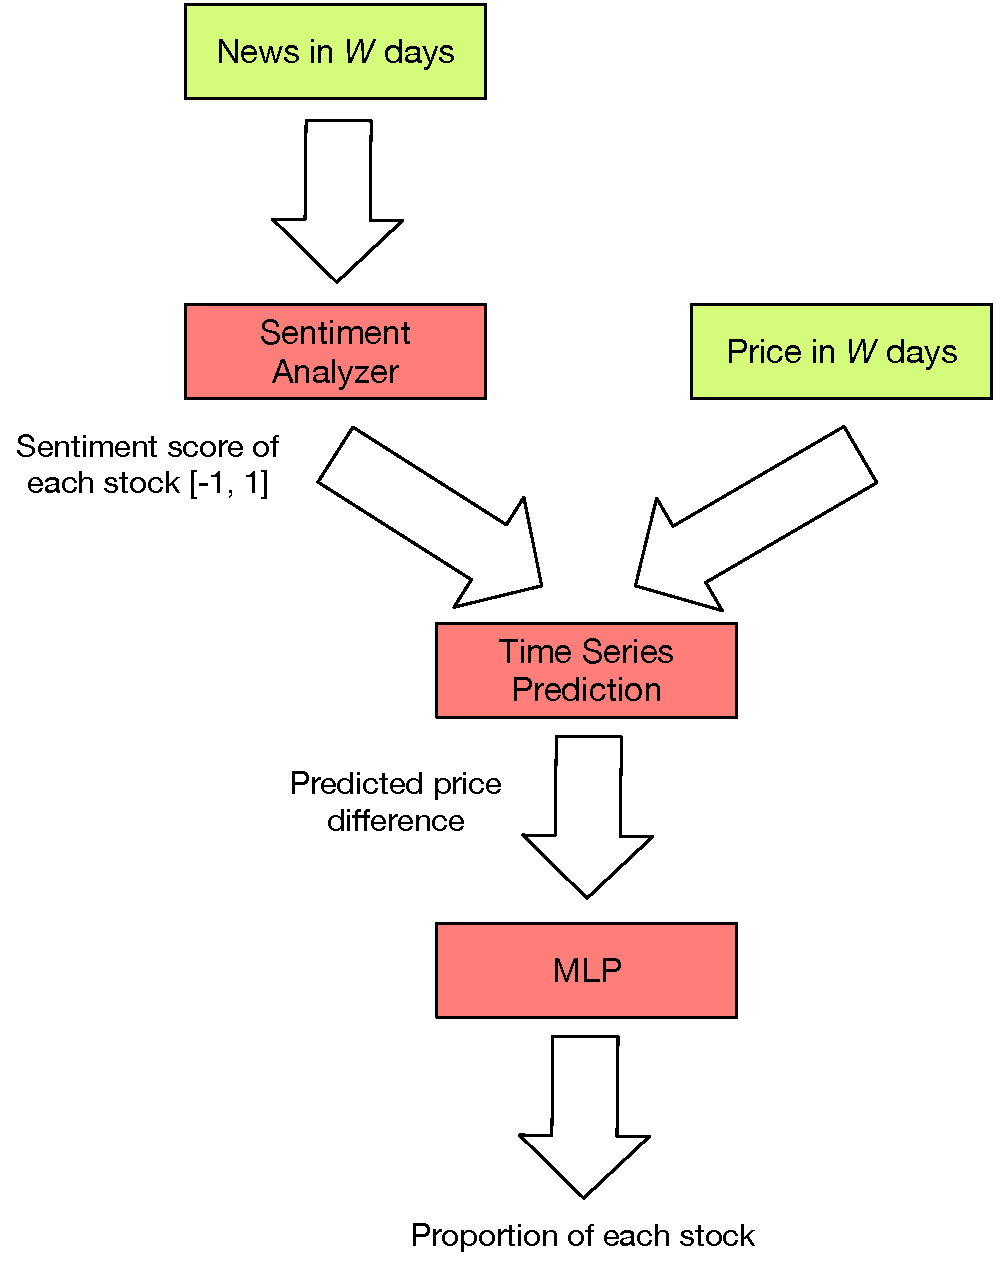
\includegraphics[width=\linewidth]{policy}
  \caption{General Policy Network Architecture}
  \label{fig:policy}
\end{figure}
We show a generic policy network in Figure~\ref{fig:policy}. The green box shows the input/output and the red box shows the network. The news data consist of a fixed number of news/tweets of $N$ stocks in one day. The price day is the open, high, low, close. 
In partially-observable sequentially decision making, we look back into $W$ days and treat all the historical price/news as observation.
The sentiment classifier takes news data as input and produce a sentiment score for each stock (probability of going up). Then, we treat the price as the original time series and sentiment score as driving series \cite{dual_attention}. The time series prediction module produces the predicted price difference. We use a final MLP to learn the final action (proportion of each stock) using RL.

\subsection{Stock Trend Prediction}
In our dataset, each day contains 25 top news. We extract the labels by comparing the stock price. If the stock price goes up, we set the label to be 1. Otherwise, we set the label to be 0.

In multi-sized window approach, we concatenate all the news into a single sentence. Our goal is to predict the stock trend by only using the news one day-ahead. Thus, it becomes a standard sentence classification problem.

In time series approach, we explore the temporal dependency by modeling the problem as non-linear auto-regressive exogenous time series prediction. We assume a pretrained sentiment scorer on universal corpus that transforms each sentence into a scalar score ranging from $[-1, 1]$ that indicates the polarity of the sentence. Then, the historical price is the original time series and sentiment scores is driving time series that affect the trend original time series. We apply a dual-stage attention mechanism that both select which driving series to pay attention to and which time step in the history to pay attention to.

\subsubsection{Multi-sized Window CNN}
Convolutional Neural Networks are extremely useful and efficient for sentence modeling \cite{kim_cnn_sentiment}. First, we use pretrained Bert \cite{bert} to initialize our embedding layer. Then, we apply multi-filter width convolution layer to extract various $n$-gram features. After that, we use max-pooling to select the most important features. Finally, we use a fully-connected layer with softmax to output the probability of the stock trend. We apply additional dropout in the embedding layer and fully-connected layers to prevent overfitting.

\begin{figure}
  \centering
  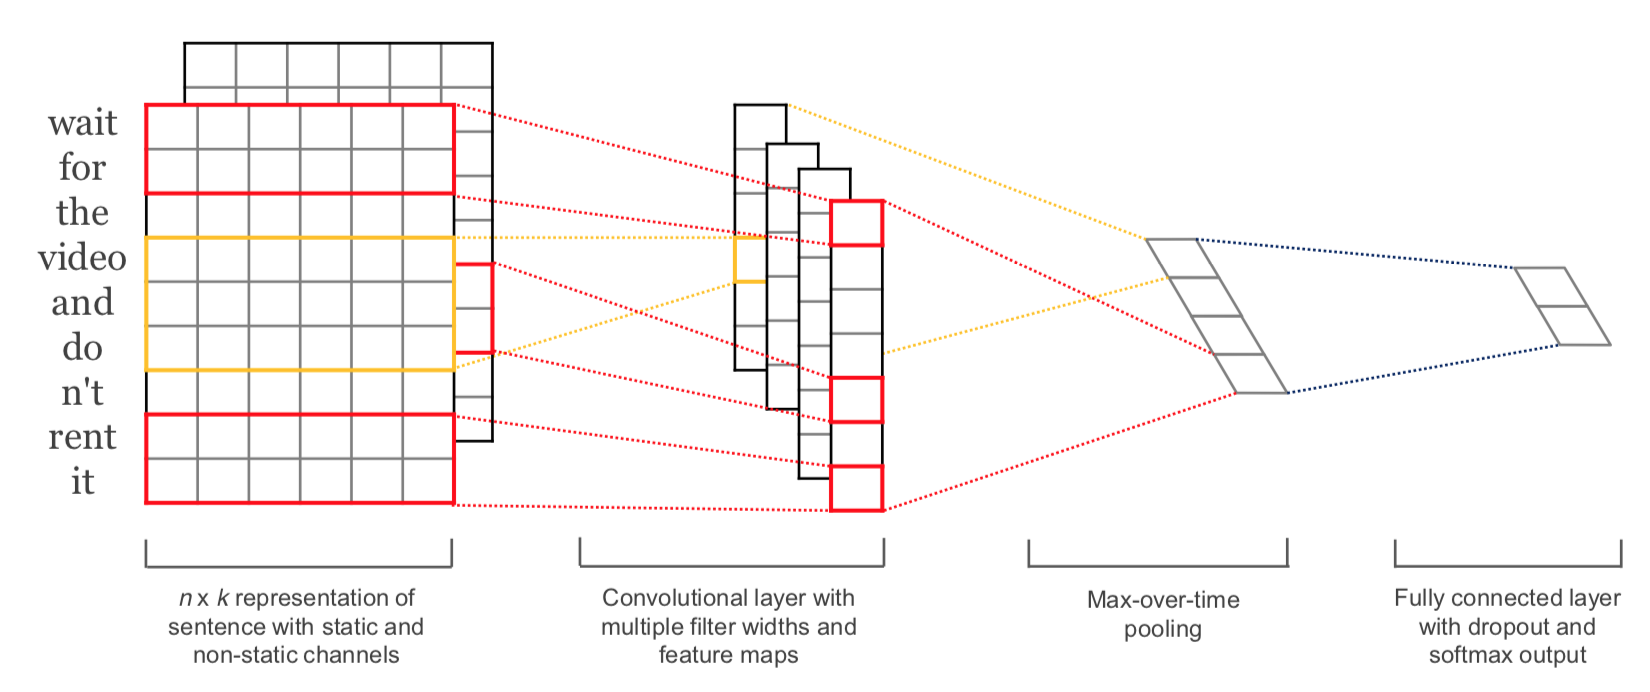
\includegraphics[width=\linewidth]{multi-size-cnn}
  \caption{Multi-sized Window CNN}
  \label{fig:multi_size_cnn}
\end{figure}

\subsubsection{Dual-Stage Attention RNN}

The architecture is borrowed from \cite{dual_attention}. In this model, assume we have $n$ driving series, which contain sentiment scores. We denote these time series as $X=(x^1, x^2, \cdots, x^n)$, each $x^i=(x^{i}_{1}, x^{i}_{2}, \cdots, x^{i}_{T-1})$, where $T$ is the window length. We also have previous values of target series $(y_1, y_2, \cdots, y_{T-1})$ with $y_t\in \mathbb{R}$. The target series in our problem is the stock price. \textbf{This model can be interpreted as we have $n$ news sources and each news source produces one news for each stock per day. We want to predict the stock trend using historical series values and news sentiment from those sources.} In the dual-stage attention-based RNN approach, for each prediction step, we select which news source and which previous time step to pay attention to.

\begin{figure}
  \centering
  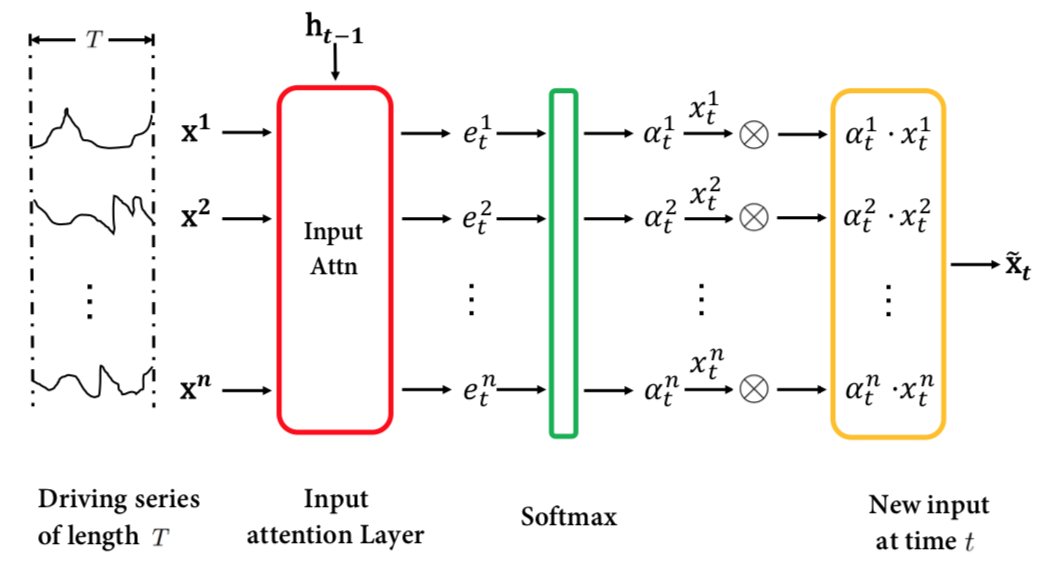
\includegraphics[width=\linewidth]{input_attention}
  \caption{Input Attention Mechanism (Figure copied with author's permission)}
  \label{fig:input_attention}
\end{figure}

\begin{figure}
  \centering
  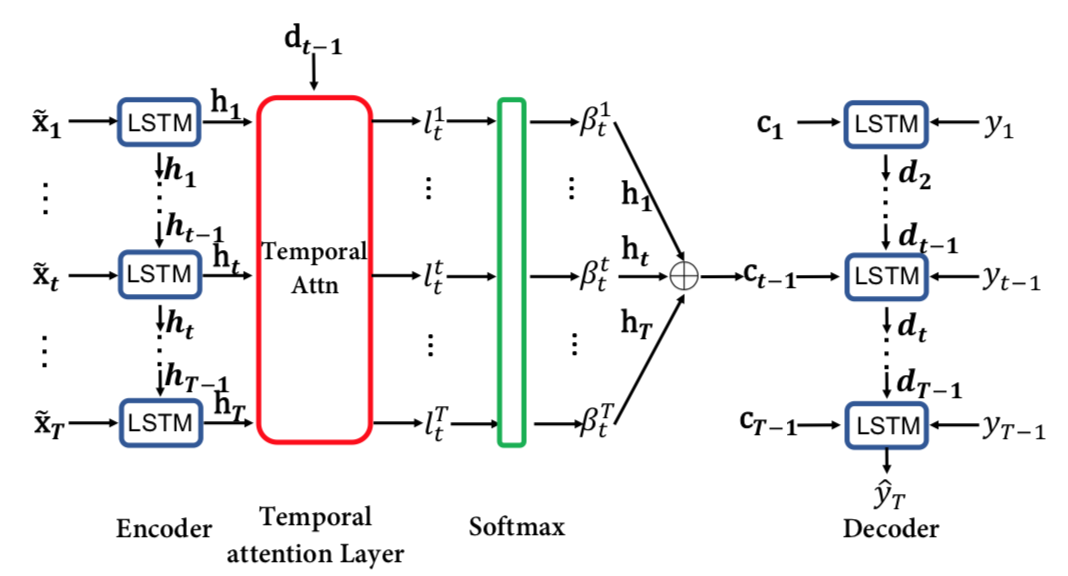
\includegraphics[width=\linewidth]{temporal_attention}
  \caption{Temporal Attention Mechanism (Figure copied with author's permission)}
  \label{fig:temporal_attention}
\end{figure}

\paragraph{Input Attention Mechanism}
We show the input attention mechanism in Figure~\ref{fig:input_attention}. The RNN model we use is LSTM \cite{lstm}. We assume $h_{t-1}$ and $s_{t-1}$ is the hidden state from previous time step, then we compute the attention weights $e_{t}^{k}$ as 
\begin{equation}
e_{t}^{k}=v_{e}^T\tanh (W_e[h_{t-1}; s_{t-1}]+U_ex^k)
\end{equation}
and
\begin{equation}
\alpha^{k}_{t}=\frac{\exp(e^{k}_{t})}{\sum_{i=1}^{n}\exp(e^{i}_{t})}
\end{equation}
$\alpha^{k}_{t}$ is the attention weight measuring the importance of the $k$-th input feature (driving series) at time $t$. With these attention weights, we can adaptively extract the driving series with $\tilde{x}_t=(\alpha^1_{t}x^1_{t}, \alpha^2_{t}x^2_{t}\cdots, \alpha^n_{t}x^n_{t})$. Then, the hidden state update at time $t$ is
\begin{equation}
h_t=\text{lstm\_cell}(h_{t-1}, \tilde{x}_t)
\end{equation}

\paragraph{Temporal Attention Mechanism}
The dual-stage attention model follows encoder-decoder framework. We show the temporal attention mechanism in Figure~\ref{fig:temporal_attention}. The decoder takes in the hidden state from the encoder, which is the input attention RNN. Then, a temporal attention mechanism is used in the decoder to adaptively select relevant encoder hidden states across all time steps. Assume the hidden state of decoder LSTM cell is $d_{t-1}$ and $s'_{t-1}$, we have
\begin{equation}
l^{i}_{t}=v^T_d \tanh(W_d[d_{t-1};s'_{t-1}]+U_dh_i)
\end{equation}
and 
\begin{equation}
\beta^i_{t}=\frac{\exp(l^{i}_{t})}{\sum_{j=1}^{T-1}\exp(l^{j}_{t})}
\end{equation}
Then, the temporal attention weight is used to combine all the encoder hidden states to form context vector as
\begin{equation}
c_t=\sum_{i=1}^{T} \beta^i_{t}h_i
\end{equation}
Once we get the context vectors, we can combine with given target series and produce the input to the LSTM cell.
\begin{equation}
\tilde{y}_{t-1} = w^T[y_{t-1};c_{t-1}] + b
\end{equation}
The newly computed $\tilde{y}_{t-1}$ is used to update the hidden state of the decoder as
\begin{equation}
d_t=\text{lstm\_cell}(d_{t-1}, \tilde{y}_{t-1})
\end{equation}
Finally, we get $d_{T-1}$ and $c_{T-1}$ after $T-1$ steps. We use another linear transform to get our final prediction as
\begin{equation}
\tilde{y}_{T}=W_y([d_T;c_T])+b
\end{equation}
For classification task, if the prediction is larger than previous time step value, we mark the stock trend as going up. Otherwise, we mark the stock trend as going down.

\subsection{Trading Strategy}
Trading strategy is the function mapping from stock prediction to final action. Given ground truth stock labels, the \textbf{optimal} action is to invest everything to the stock with highest return. In fact, \textbf{training imitation learning agent mapping directly from news to optimal action is equivalent to only predicting the probability of stock goes up/down.} The action can be computed by only investing to the stock with highest probability that price will go up. However, investing all the money into one stock is very risk. In this section, we propose several na\"ive strategy and a strategy using reinforcement learning.
\subsubsection{Na\"ive Strategy}
We propose an na\"ive strategies using trust-region investment: assume the probability of $N$ stocks (including cash) going up is $p_1, p_2, \cdots, p_N$, then if $p_i < threshold$, set $p'_i=0$. Otherwise, $p'_i=p_i$. Then, $a_i=\frac{p'_i}{\sum_{j=1}^{N}p'_j}$. The idea is that we only invest when the system is very certain about the trend. Note that we set the probability of cash going up to be 0.5. Thus, if all the stock goes down, we will not invest in any stocks. In our experiments, we set threshold to be 0.7, 0.8, 0.9.
\subsubsection{RL-based Strategy}
Instead of developing custom strategy, we apply reinforcement learning to learn policy directly using policy gradient on historical data. Vanilla policy gradient suffers from low sample efficiency. In this work, we apply proximal policy optimization that optimize the following surrogate loss
\begin{equation}
L^{CLIP}(\theta)=\hat{\mathbb{E}}_t[\min(r_t(\theta)\hat{A}_t, \text{clip}(r_t(\theta), 1-\epsilon, 1+\epsilon))]
\end{equation}
where $r_t=\frac{\pi_\theta(a_t|s_t)}{\pi_{\theta_{old}}(a_t|s_t)}$ is the probability ratio between new policy and old policy and $\hat{A}_t$ is the estimated advantage function. We show the algorithm in Figure~\ref{fig:ppo}.
\begin{figure}
  \centering
  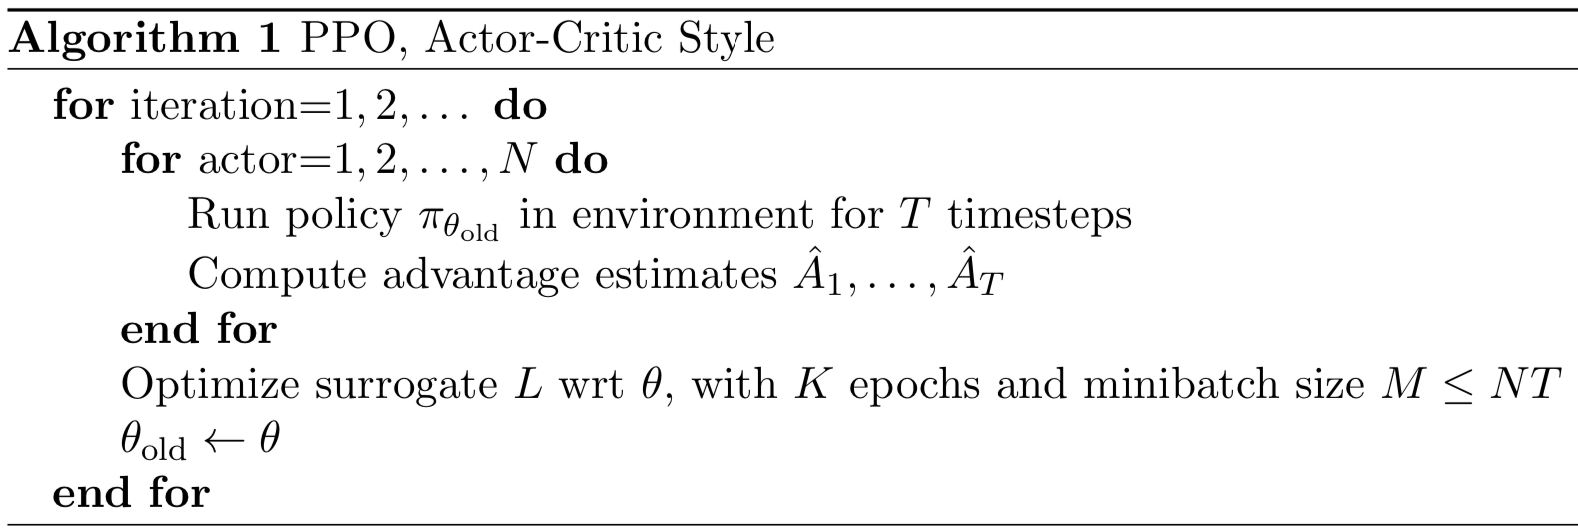
\includegraphics[width=\linewidth]{ppo}
  \caption{Proximal Policy Optimization}
  \label{fig:ppo}
\end{figure}


\section{Experimental Setup}
\subsection{Datasets}
We use Dow Jones Industrial Average (DJIA) dataset from \url{https://www.kaggle.com/aaron7sun/stocknews}. It contains DJIA price from 2008-08-08 to 2016-07-01. For each day, it also contains 25 top news headline. We label the data using the trend (up/down) of tomorrow's closing price. We split the whole data to 0.8/0.2 as training/test data.

\subsection{Performance Metrics}
To evaluate stock trend prediction, we use binary F1-score. The confusion matrix is defined in Table~\ref{table:confusion}. Precision is defined as $$\text{Precision}=\frac{\text{TP}}{\text{TP}+\text{FP}}$$ and recall is defined as 
$$\text{Recall}=\frac{\text{TP}}{\text{TP}+\text{FN}}$$
The binary F1-score is simply
$$\text{F1-score}=\frac{2\cdot\text{Precision}\cdot\text{Recall}}{\text{Precision}+\text{Recall}}$$
\begin{table*}
  \centering
  \caption{Confusion Matrix of Binary Classification}
  \begin{tabular}{|c|c|c|}
    \hline
    & Predicted True & Predicted False \\\hline
    Actual True & True Positive (TP) & False Negative (FN) \\\hline
    Actual False & False Positive (FP) & True Negative (TN) \\\hline
  \end{tabular}
  \label{table:confusion}
\end{table*}

To evaluate the trading performance, we calculate the return defined in Eq~\ref{eq:profit_mu}.

\section{Results}

\subsection{Stock Trend Prediction}
%\begin{table*}
%  \centering
%  \caption{Stock Trend Prediction Result}
%  \begin{tabular}{|c|c|c|}
%    \hline
%    Method & Multi-sized Window CNN & Dual-Stage Attention RNN \\\hline
%    F1-score &  0.6021  &  \\\hline
%  \end{tabular}
%  \label{table:stock_trend_prediction}
%\end{table*}

\subsubsection{Multi-sized CNN}
The window size we choose is $3, 4, 5, 6, 7, 8$. We show a training/val loss in Figure~\ref{fig:multi_size_cnn_loss} and accuracy/recall/f1 in Figure~\ref{fig:multi_size_cnn_stats}. We observed that the validation loss diverges at the beginning of the training, indicating the model actually doesn't even learn anything from training data that can be generalized to validation data. The model starts to overfit the training data at the beginning of the training procedure.

\begin{figure}
  \centering
  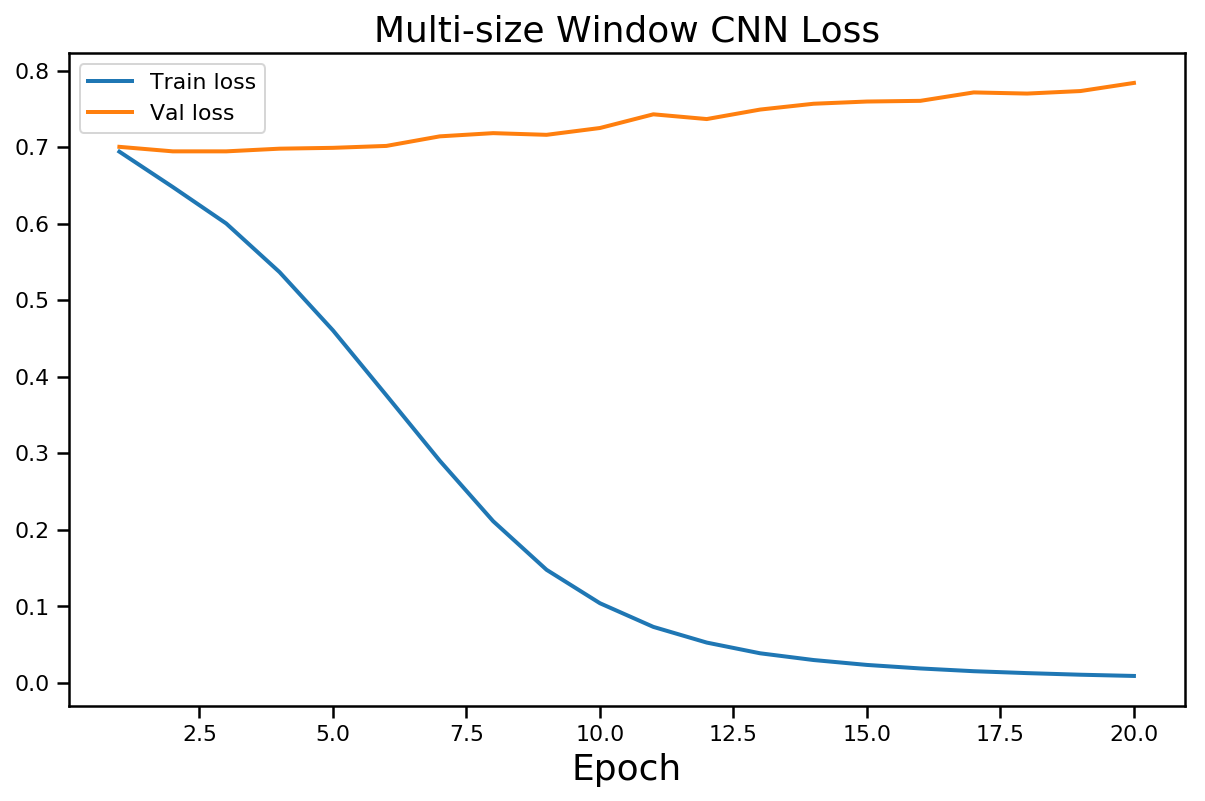
\includegraphics[width=\linewidth]{multi_size_cnn_loss}
  \caption{Multi-size CNN Loss}
  \label{fig:multi_size_cnn_loss}
\end{figure}

\begin{figure}
  \centering
  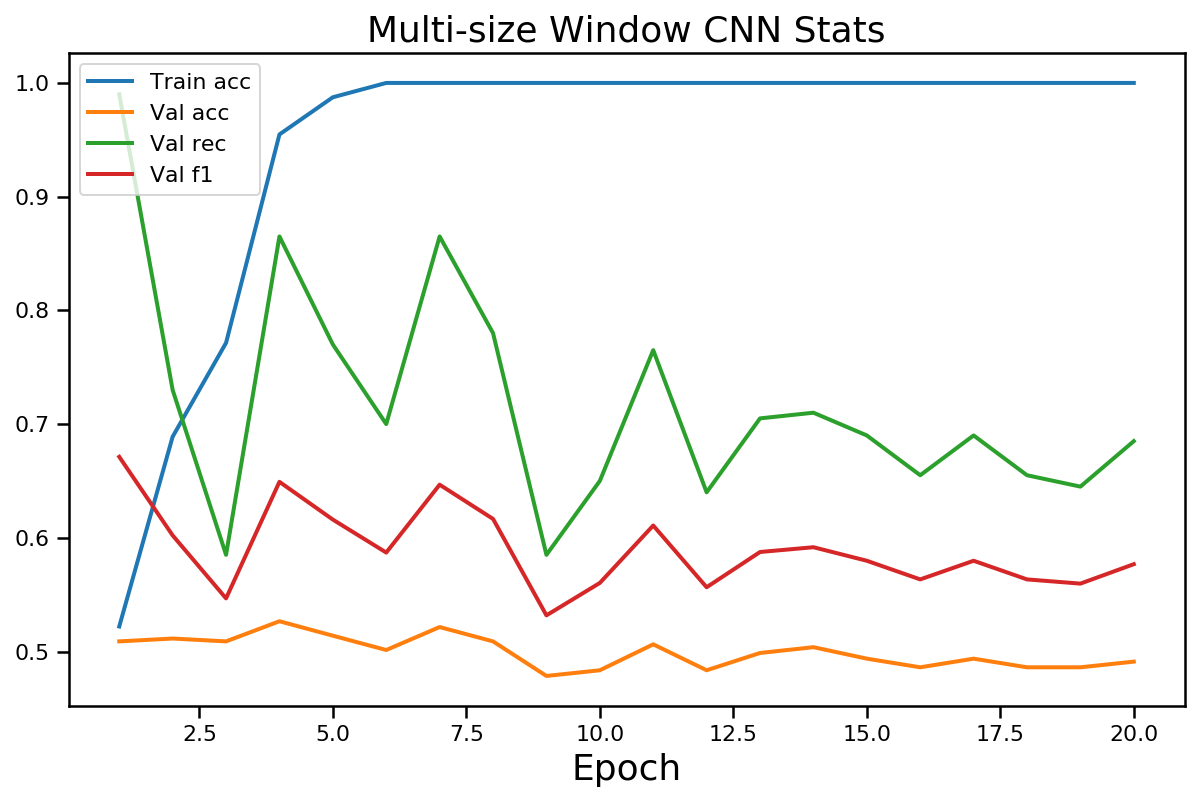
\includegraphics[width=\linewidth]{multi_size_cnn_stats}
  \caption{Multi-size CNN Statistics}
  \label{fig:multi_size_cnn_stats}
\end{figure}


\subsubsection{Dual-Stage Attention RNN}
We use NLTK \cite{nltk} open source SentimentIntensityAnalyzer to extract the sentiment polarity of a sentence. We show the loss of window length 3 and 5 in Figure~\ref{fig:dual_attention_window_3} and Figure~\ref{fig:dual_attention_window_5}, respectively. The same problem persists here that the validation loss diverges at the beginning of the training procedure.

\begin{figure}
  \centering
  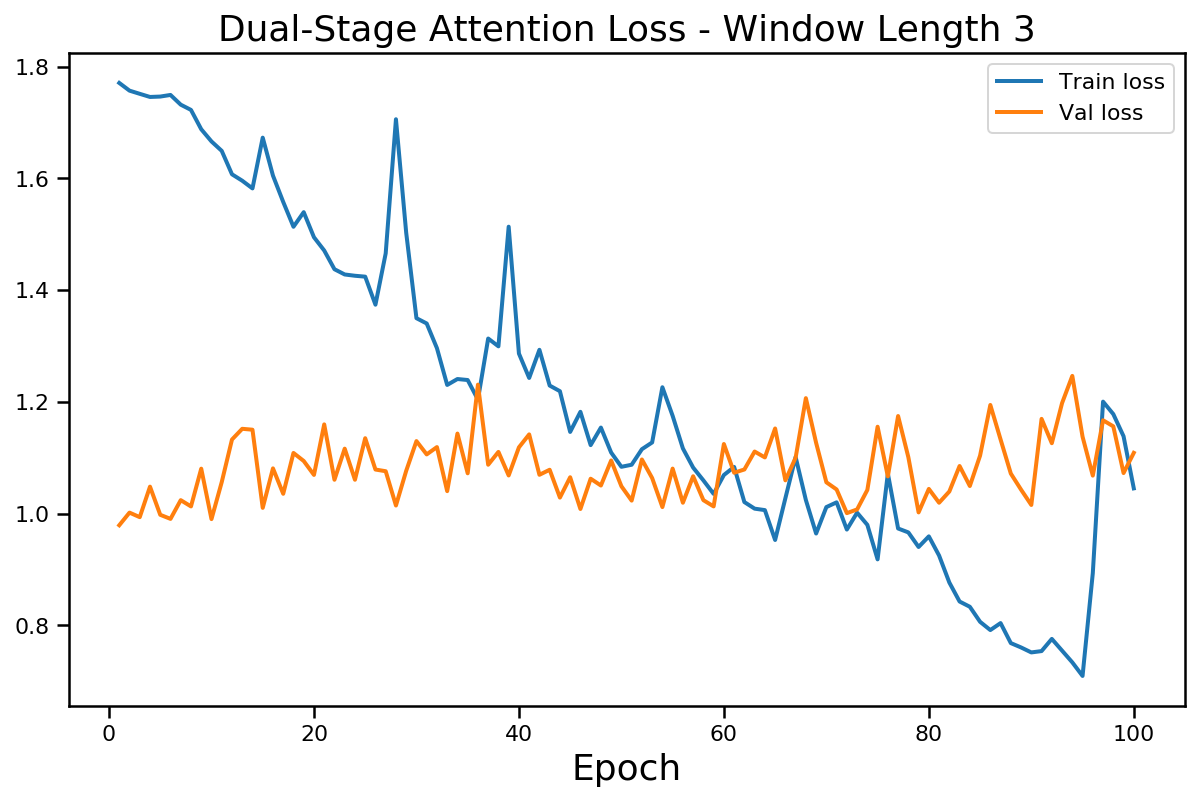
\includegraphics[width=\linewidth]{dual_attention_window_3}
  \caption{Dual-Stage Attention Loss Window 3}
  \label{fig:dual_attention_window_3}
\end{figure}

\begin{figure}
  \centering
  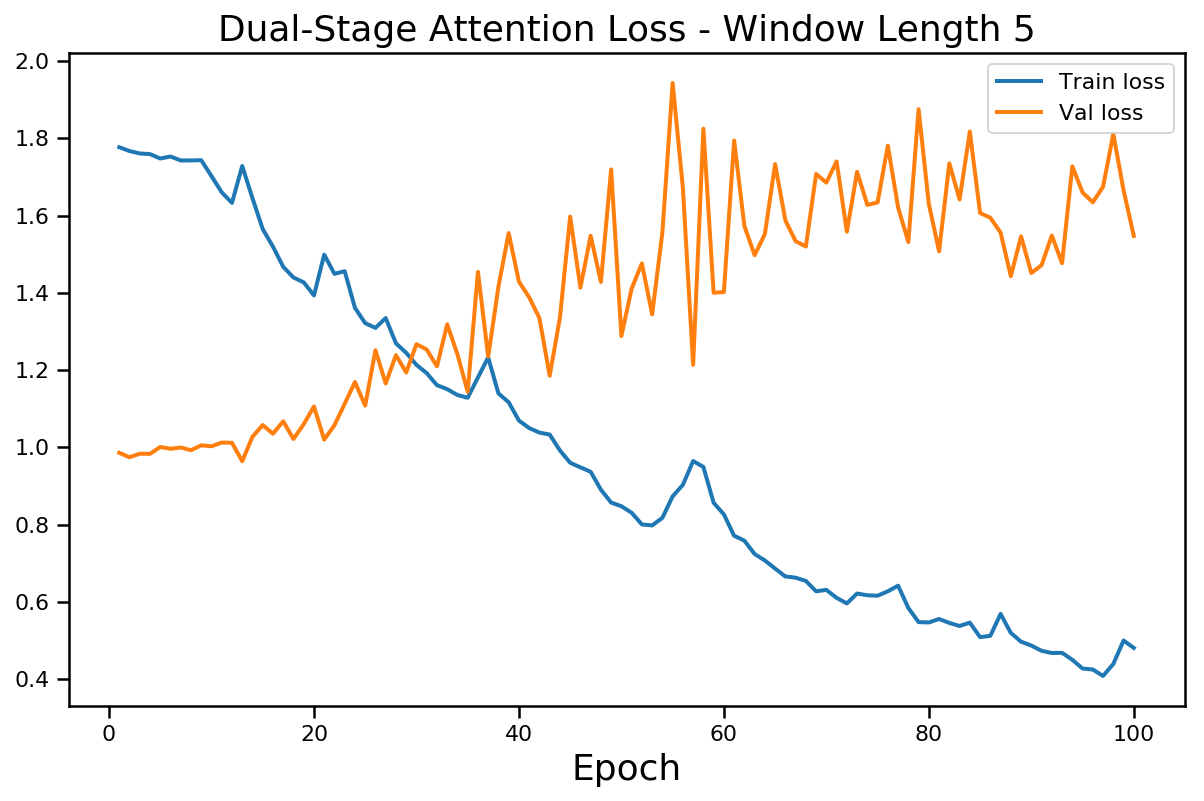
\includegraphics[width=\linewidth]{dual_attention_window_5}
  \caption{Dual-Stage Attention Loss Window 5}
  \label{fig:dual_attention_window_5}
\end{figure}


\subsection{Trading Performance}
We run various policy including trust-region investment, running statistics and RL-based strategy on test data and show the trading performance in Table~\ref{table:trading_performance}. We show portfolio value versus market value of PPO-based approach and trust-region based approach (0.7) in Figure~\ref{fig:ppo_trading} and Figure~\ref{fig:trust_region_trading}. We show that in RL-based approach, we can achieve slightly higher return than market value while in trust-region based approach, we always hold the money without investing in any stock. This is due to the fact that the performance of predictor is really bad and it always produces probability around 0.5.

\begin{table*}
  \centering
  \caption{Average Trading Performance on 100 runs}
  \begin{tabular}{|c|c|c|c|c|}
    \hline
    Method & Trust-region (0.7) & Trust-region (0.8) & Trust-region (0.9) & PPO \\\hline
    Return & 1.0  & 1.0 & 1.0 &  1.006 \\\hline
  \end{tabular}
  \label{table:trading_performance}
\end{table*}

\begin{figure}
  \centering
  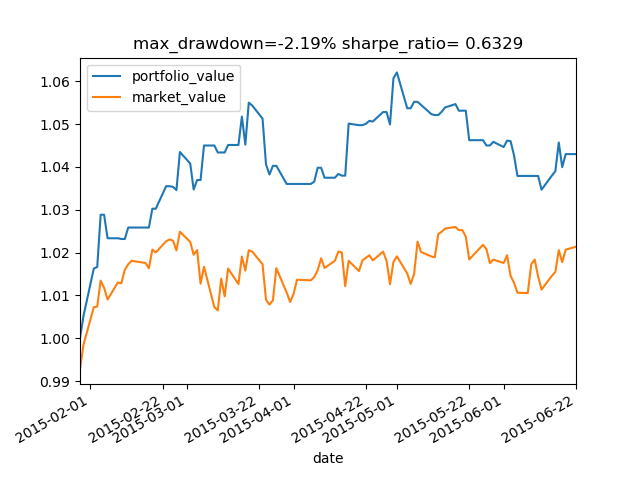
\includegraphics[width=\linewidth]{ppo_trading}
  \caption{Trading Performance of PPO}
  \label{fig:ppo_trading}
\end{figure}

\begin{figure}
  \centering
  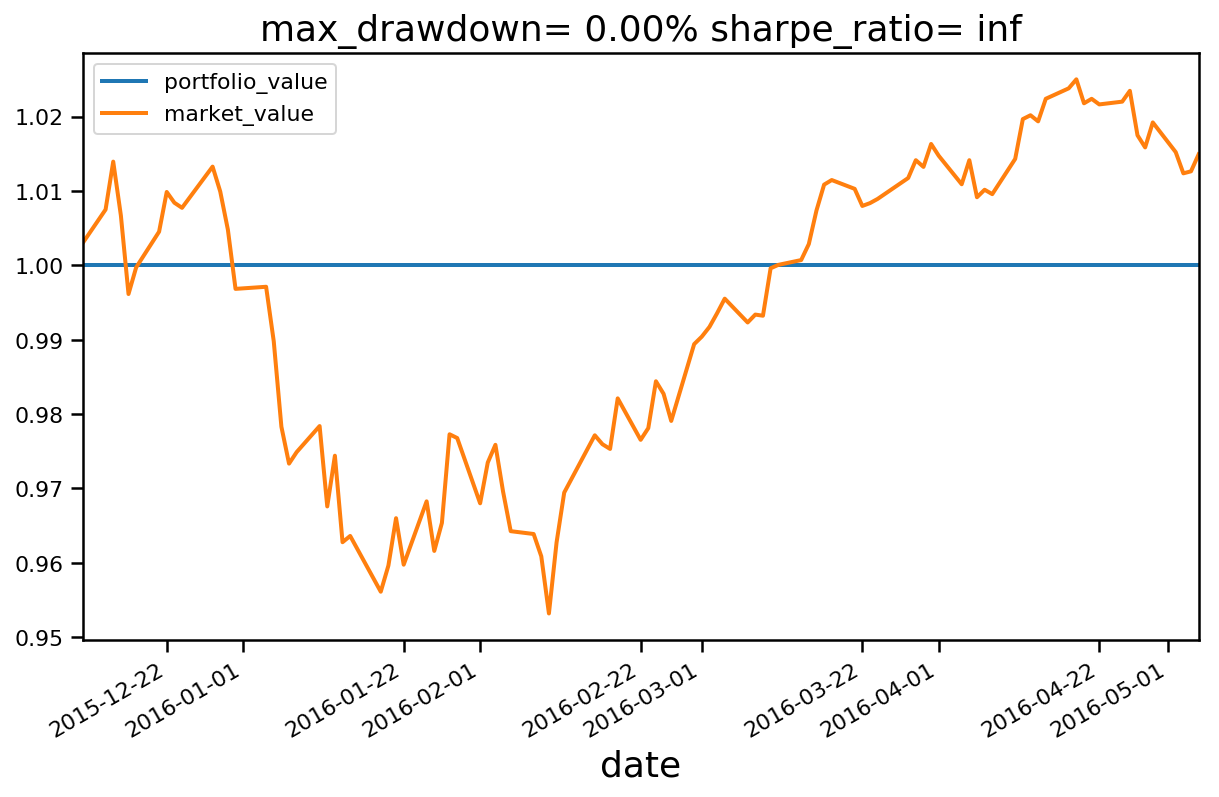
\includegraphics[width=\linewidth]{trust_region_trading}
  \caption{Trading Performance of Trust Region Policy (0.7)}
  \label{fig:trust_region_trading}
\end{figure}


\section{Discussions}
In this report, we explore several natural language models that extract the sentence sentiment features to predict the stock trend and make appropriate actions. However, none of those approaches finally works. We doubt the validity of these dataset. We try to manually label the sentiment. We label the sentence as 1 if there is a positive relationship between the sentence and the stock, 0 if there is no relationship and -1 if there is negative relationship. We found that most the sentences, even to human, is extremely vague how they would affect the stock trend.
\begin{itemize}
  \item UK Hospitals Are Feeding 1.6 Million Patients Health Records to Googles AI: Positive
  \item Final warning to Facebook by Frances data watchdog: Negative
  \item Iran wants India to pay oil dues in euros: Unknown
  \item IMF chief backs Athens as permanent Olympic host: Unknown
  \item Chinese oil pipeline explodes: Negative
  \item India gets \$1 billion loan from World Bank for solar mission: Unknown
\end{itemize}
We realized that in this problem, the method is actually secondary. The data source matters a lot. We will try to build an efficient tweets/news scrapper that extract most relevant features in future work.

\bibliography{bib/acl2019}
\bibliographystyle{acl_natbib}

%\appendix
%
%\section{Appendices}
%TODO


\end{document}
